\section{Results}
\subsection{Relaxation time}
The variation of parameter $\tau$ in the spin-echo and 180°-90° sequence allowed us to measure the time evolution of the transverse, Fig. \ref{fig:GD500 T2 Sp} \& Fig. \ref{fig:GD600 T2 Sp}, and anti-parallel magnetization, Fig. \ref{fig:GD500 T1} \& Fig. \ref{fig:GD600 T1}. A second measurement for the transverse component using the Carr-Purcell sequence delivered Fig. \ref{fig:GD500 T2 CP} \& Fig. \ref{fig:GD600 T2 CP}. 

\begin{figure}[!htbp]
  \centering
  \begin{subfigure}[b]{0.45\textwidth}
    \centering
    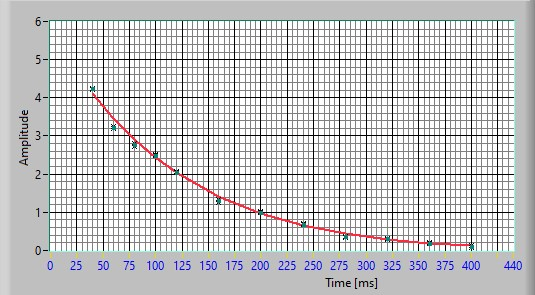
\includegraphics[width=\textwidth]{./Protocol images/GD500_T2_sp_fit (1).jpg}
    \caption{GD500}
    \label{fig:GD500 T2 Sp}
  \end{subfigure}
  \hfill
  \begin{subfigure}[b]{0.45\textwidth}
    \centering
    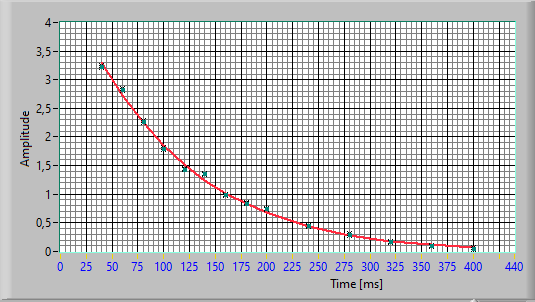
\includegraphics[width=\textwidth]{./Protocol images/GD60_Sp (1).png}
    \caption{GD600}
    \label{fig:GD600 T2 Sp}
  \end{subfigure}
  \caption{Decay curve of $M_\perp$ measured with spin-echo methode}
  \label{fig:subsidebyside}
\end{figure}

\begin{figure}[!htbp]
  \centering
  \begin{subfigure}[b]{0.45\textwidth}
    \centering
    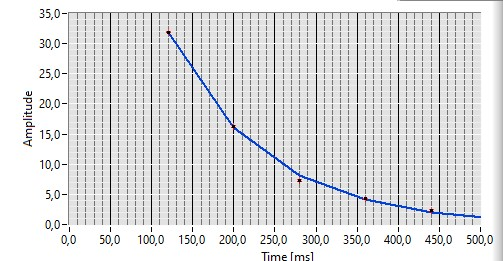
\includegraphics[width=\textwidth]{./Protocol images/GD500_T2_cp_fit.jpg}
    \caption{GD500}
    \label{fig:GD500 T2 CP}
  \end{subfigure}
  \hfill
  \begin{subfigure}[b]{0.45\textwidth}
    \centering
    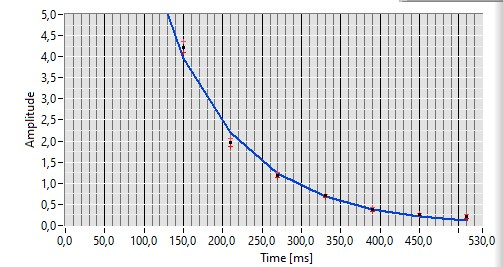
\includegraphics[width=\textwidth]{./Protocol images/GD600_CP_fit (1).jpg}
    \caption{GD600}
    \label{fig:GD600 T2 CP}
  \end{subfigure}
  \caption{Decay curve of $M_\perp$ measured with Carr-Purcell sequence}
  \label{fig:subsidebyside}
\end{figure}

\begin{figure}[!htbp]
  \centering
  \begin{subfigure}[b]{0.45\textwidth}
    \centering
    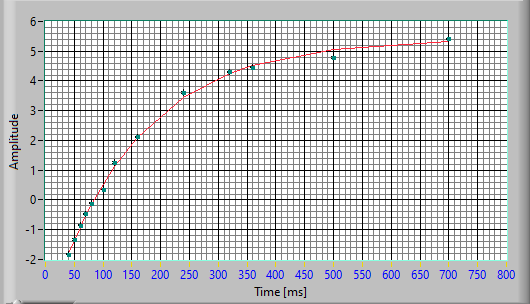
\includegraphics[width=\textwidth]{./Protocol images/GD500_T1 (1).png}
    \caption{GD500}
    \label{fig:GD500 T1}
  \end{subfigure}
  \hfill
  \begin{subfigure}[b]{0.45\textwidth}
    \centering
    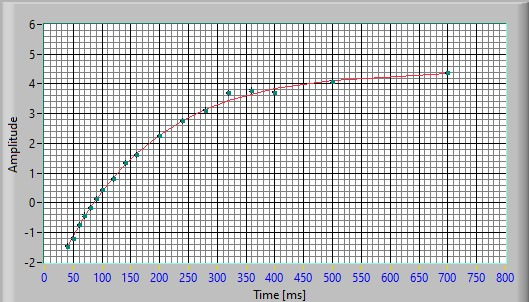
\includegraphics[width=\textwidth]{./Protocol images/GD600_T1 (1).jpg}
    \caption{GD600}
    \label{fig:GD600 T1}
  \end{subfigure}
  \caption{Decay curve of $M_\parallel$ measured with 180°-90° sequence}
  \label{fig:subsidebyside}
\end{figure}
A quick glance at the curves already tell  us that the time evolution of the components of the magnetization describe a decay curves, as we expected from the solutions of the bloch equations,  eq.\ref{eq: sol. bloch T1} \& eq. \ref{eq: sol. bloch T2}. By fitting these equation to our data we are able to find the characteristic relaxation times $T_1$ and $T_2$. See Tab. \ref{tab: relaxation times}.
\begin{table}[!htbp]
 \begin{center}
  \caption{Relaxation times for Gd500 and Gd600}
  \label{tab: relaxation times}
  \begin{tabular}{|c||c|c|c|c|}
	\hline
	\multirow{2}{*}{\textbf{Probe}} & \multicolumn{3}{c}{spin-spin $T_2$ [ms]} &\multirow{2}{*}{ spin-lattice $T_1$[ms]}\\
	& spin-echo & Carr-Purcell & deviation $\sigma$\\
	\hline
	\hline	
	Gd 500 & 110 $\pm$ 6 & 111,3 $\pm$ 1,5 & 0,5 & 159 $\pm$ 1,3 \\
	Gd 600 & 115,7 $\pm$ 1,2 & 116,9 $\pm$ 0,9 & 0,8 & 154,4 $\pm$ 1,2 \\
	\hline
  \end{tabular}
 \end{center}
\end{table}

Firstly we observe that the spin-spin relaxation time of the probe with higher density, GD600, is larger than that of GD500, which contradicts our expectations. From our theory we know that $T_2$ is mainly determined by the interaction between the proton's spins. Hence the bigger the concentration, which translates to a larger amount of protons therefore of spins, the  more possibilities there exist for a proton to dissipate its excitation energy resulting in a smaller spin-spin relaxation time. 
Secondly we observe that $T_{1, Gd500}$ \> $T_{1,Gd600}$, as we expected. Analogously to the case of $T_2$, a higher concentration also translates in a smaller spin-lattice relaxation time, since the excited state has a larger lattice in which it can dissipates its energy.


From our experiment we can observe that the deviation between the results gained by the spin-echo and Carr-Purcell methods are not significant, however from our theory we know that this second method delivers more exact results. The Carr-Purcell sequence is also a faster measurement technique since it can be completely automatized, thus reducing the susceptibility to human errors. Lastly we also observe a higher precision from this second method, it delivers a smaller uncertainty in all measurements. This last point is better observed by the measurements of Gd500 where the uncertainty of the spin-echo method is almost 4 times bigger than the one delivered by the Carr-Purcell sequence. 
\subsection{Chemical shift}
The measured frequency spectra for the samples with and without the reference substance are to be seen in Fig.\ref{fig:sample A} - Fig. \ref{fig:sample E}.
\begin{figure}[!htbp]
  \centering
  \begin{subfigure}[b]{0.47\textwidth}
    \centering
    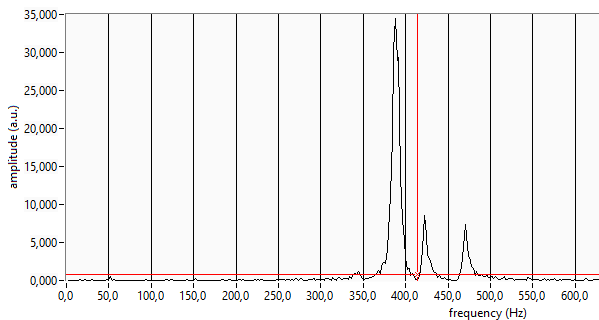
\includegraphics[width=\textwidth]{./Latex images/A.png}
    \caption{Substance A}
    \label{fig: A}
  \end{subfigure}
  \hfill
  \begin{subfigure}[b]{0.47\textwidth}
    \centering
    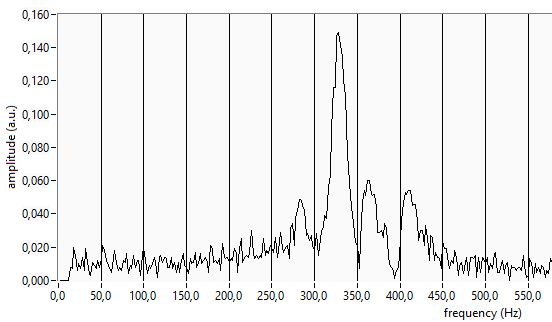
\includegraphics[width=\textwidth]{./Latex images/Ap.png}
    \caption{Substance A + TMS}
    \label{fig: A + TMS}
  \end{subfigure}
  \caption{Frequency spectrum of substance A}
  \label{fig:sample A}
\end{figure}

\begin{figure}[!htbp]
  \centering
  \begin{subfigure}[b]{0.47\textwidth}
    \centering
    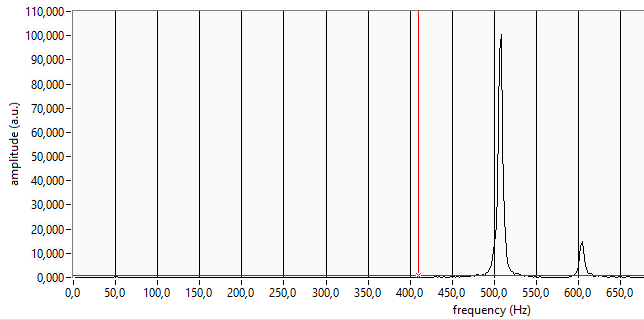
\includegraphics[width=\textwidth]{./Latex images/B.png}
    \caption{Substance B}
    \label{fig: B}
  \end{subfigure}
  \hfill
  \begin{subfigure}[b]{0.47\textwidth}
    \centering
    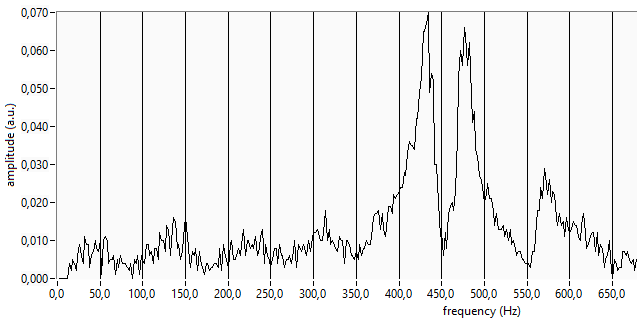
\includegraphics[width=\textwidth]{./Latex images/Bp.png}
    \caption{Substance B + TMS}
    \label{fig: B + TMS}
  \end{subfigure}
  \caption{Frequency spectrum of substance B}
  \label{fig:sample B}
\end{figure}


\begin{figure}[!htbp]
  \centering
  \begin{subfigure}[b]{0.47\textwidth}
    \centering
    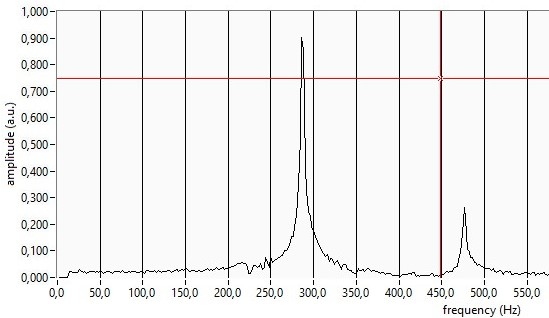
\includegraphics[width=\textwidth]{./Latex images/C.jpg}
    \caption{Substance C}
    \label{fig: C}
  \end{subfigure}
  \hfill
  \begin{subfigure}[b]{0.47\textwidth}
    \centering
    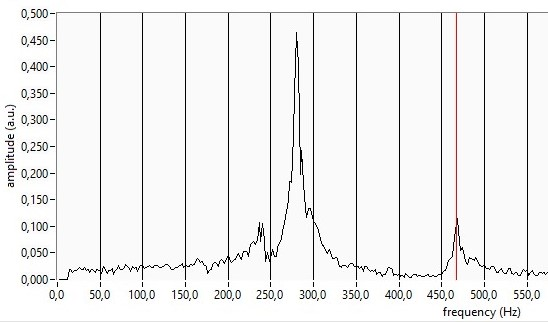
\includegraphics[width=\textwidth]{./Latex images/Cp.jpg}
    \caption{Substance C + TMS}
    \label{fig: C + TMS}
  \end{subfigure}
  \caption{Frequency spectrum of substance C}
  \label{fig:sample C}
\end{figure}

\begin{figure}[!htbp]
  \centering
  \begin{subfigure}[b]{0.47\textwidth}
    \centering
    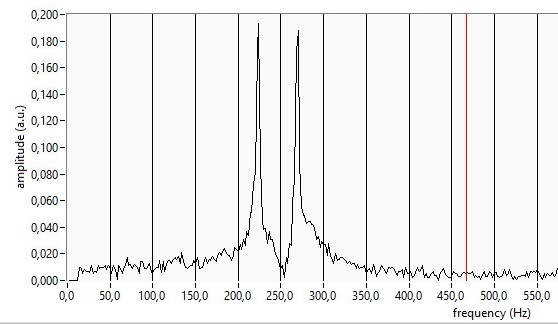
\includegraphics[width=\textwidth]{./Latex images/D.jpg}
    \caption{Substance D}
    \label{fig: D}
  \end{subfigure}
  \hfill
  \begin{subfigure}[b]{0.47\textwidth}
    \centering
    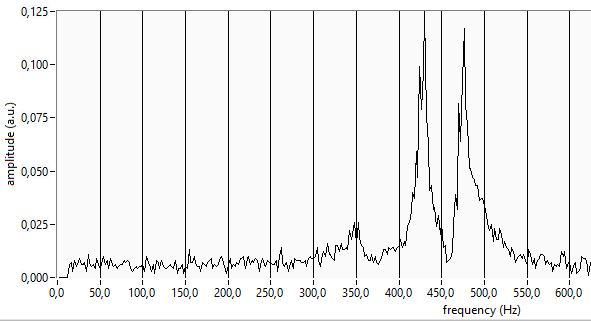
\includegraphics[width=\textwidth]{./Latex images/Dp.png}
    \caption{Substance D + TMS}
    \label{fig: D + TMS}
  \end{subfigure}
  \caption{Frequency spectrum of substance D}
  \label{fig:Sample D}
\end{figure}


\begin{figure}[!htbp]
  \centering
  \begin{subfigure}[b]{0.47\textwidth}
    \centering
    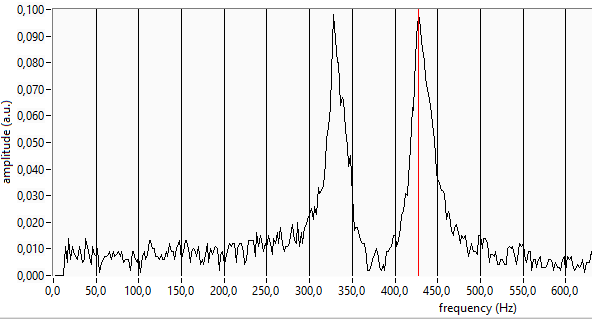
\includegraphics[width=\textwidth]{./Latex images/E.png}
    \caption{Substance E}
    \label{fig: E}
  \end{subfigure}
  \hfill
  \begin{subfigure}[b]{0.47\textwidth}
    \centering
    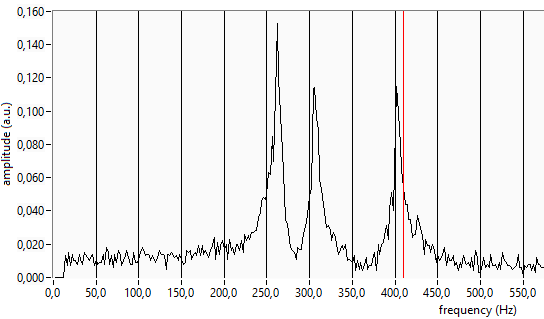
\includegraphics[width=\textwidth]{./Latex images/Ep.png}
    \caption{Substance E + TMS}
    \label{fig: E + TMS}
  \end{subfigure}
  \caption{Frequency spectrum of substance E}
  \label{fig:sample E}
\end{figure}

The measured relative distances between the maximum of  TMS and the active groups of the probes are in Tab. \ref{tab: identification} along with then name of the molecule matching the found active groups.
\begin{table}[!htbp]
 \begin{center}
  \caption{ Measured relative chemical and identification of probes}
  \label{tab: identification}
  \begin{tabular}{|c||c|c|c|c|}
  \hline
 	\multirow{2}{*}{\textbf{Probe}} & \multicolumn{3}{c}{Relative distance $\Delta$ [ppm]} &\multirow{2}{*}{ \textbf{Substance}} \\
								   &	 $\Delta_1$ & $\Delta_2$ &  $\Delta_3$ & \\
\hline
\hline
 	A & 2,3 & 4,1 & 6,8& fluroacetone \\
 	B & 2,5 & 7,2 & - & p-xylol \\
 	C & 2,2 & 11,8& - & acetic acid \\
 	D & 4,1 & 6,5 & - & fluroacetonitril \\
 	E & 2,3 & 7,1 & - & toluol \\
 	\hline
  \end{tabular}
 \end{center}
\end{table}
In the given list of molecules,see Fig. \ref{fig: identification}, we notice that fluroacetone is the only molecule with three maxima in its spectrum. Given its chemical components we expect one maximum corresponding to $CH_3$ and two lines from $FH_2$. This line splitting arise from the extra magnetic energy given to this component. Therefore to identify probe A there is no need to measure the relative distances $\Delta_i$ meticulously, instead a qualitative study of its spectrum, Fig. \ref{fig:sample A} is sufficient to identify it as fluroacetone. 
A study o f the measured relative chemical shift of $D$ shows that it contains the 2 lines from $FH_2$ which leads us to identify it as fluroacetonitril.  
On the other hand, we can see in Tab. \ref{tab: identification} that probes $B$ and $E$ have the same active groups, however we see a higher intensity in the peak corresponding to the active group $CH_3$ in the spectra of probe B, Fig. \ref{fig: B}, in comparison to that shown in $E$'s spectra, Fig. \ref{fig: E}. With this observation we are able to identify substance $B$ as p-xylol and $E$ as toluol. 
Lastly we identify probe $C$ as acetic acid due to the big chemical shift $\Delta_2$, which is caused by the active group $COOH$
\subsection{Imaging}
\paragraph{1 dimensional imaging}
The signal obtained by a vertical imaging of two probe tubes containing the same oil show disparities, see Fig. \ref{fig: long and short oil}. In the vial with less volume we see a constant signal, with some noise on top of it, meanwhile we observe a increase in the signal of the vial with higher volume of oil in range $x < -15$ mm and $x > 15$ mm. This sudden change in the measured signal is an effect caused by the non-linearity of the field gradient. It is know that the applied magnetic field is not perfectly linear. In conclusion, the probes have to be set in a position $x \in [-15$ mm, $15$ mm$]$ in order to minimize the the effect of non-linearity of the field gradient. 
\begin{figure}[!htbp]
  \begin{center}
    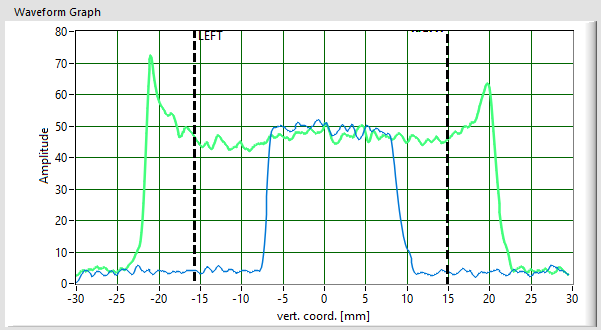
\includegraphics[width= 0.6\textwidth]{./Protocol images/III/long&short_signal.png}
 \caption{1 dimensional NMRI of 2 oil samples. Blue line: short oil sample, green line: long oil sample}
    \label{fig: long and short oil}
   \end{center}
 \end{figure} 
 
Secondly we insert a probe tube containing oil and a piece of teflon. The measured vertical profile, see Fig. \ref{fig:teflon}, show a pattern of peaks and valleys which give us information about the structure of the teflon piece. Teflon does not emit an NMR signal, thus the pattern shown in the measured signal indicate that the used piece consists of stacked teflon plates. The valleys are generated by the presence of said plates. In this areas the signal is not zero since there still oil around the probe which does emit a NMR signal. In the other hand the peaks represent the areas where the plates are bonded to one another, and due to the higher volume of oil in such areas the measured signal is stronger.  

\begin{figure}[!htbp]
  \begin{center}
    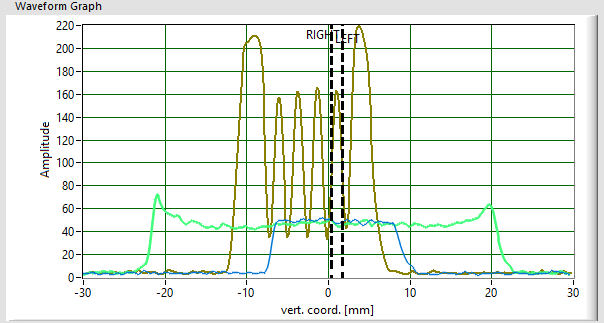
\includegraphics[width= 0.6\textwidth]{./Protocol images/III/three_profiles.png}
 \caption{1 dimensional NMRI of 2 oil samples \& Teflon. Blue: short oil sample, green: long oil sample, brown: Teflon}
    \label{fig:teflon}
   \end{center}
 \end{figure} 
\paragraph{Time evolution of system}
The vertical profile was measured in a time span of 96s. The NRM signal for times $t = 1,10, 30, 50, 96$ are plotted in Fig. \ref{fig:time evolution system}. In this diagram we observe how the position curve develops a concavity. We remember that the diffusion equation,
\begin{equation}
\frac{\partial u}{\partial t} = D\frac{\partial^2 u}{\partial x^2}
\end{equation}
describes a convex curve. Therefore we conclude that the oil pouring down through the sand is not a diffusion process. Instead, the found time evolution is proper of a percolation process, which describes the movement and filtering of fluids through porous materials. 
\begin{figure}[!htbp]
  \begin{center}
    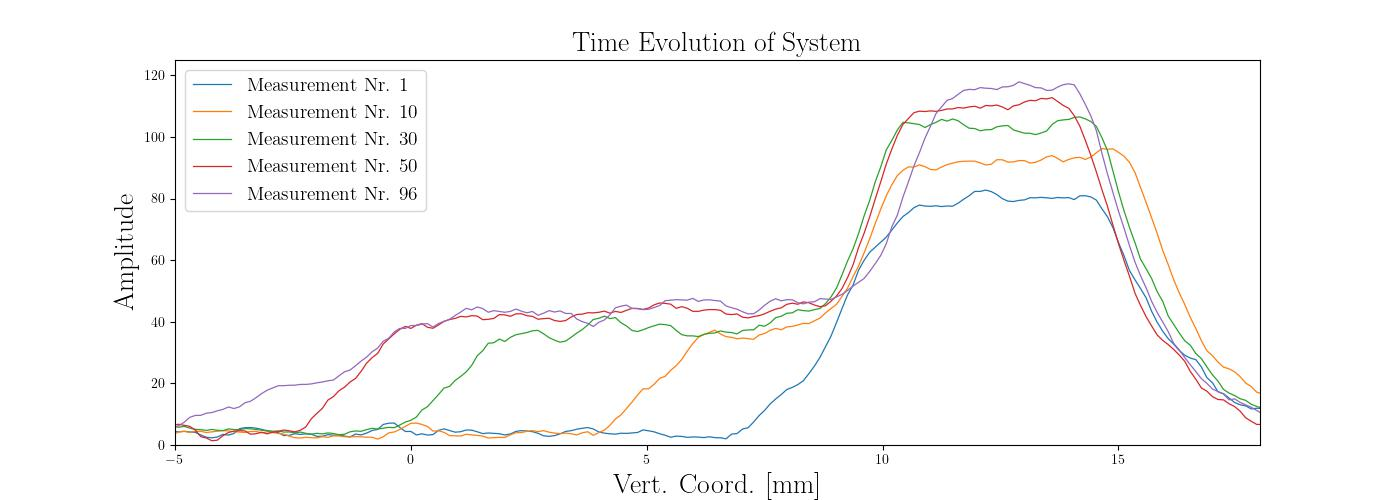
\includegraphics[width= 1.0\textwidth]{./Latex images/time_evolution.jpg}
 \caption{Time evolution of sand and oil probe.}
    \label{fig:time evolution system}
   \end{center}
 \end{figure}
\paragraph{2 dimensional imaging}
For the 2D imaging we used a steam of celery, a peanut and a pecan peanut. 
When studying the peanut we first observe that due to the lack of water or fat in the nut's shell, it does not emit any NMR. Hence, in the taken scan we can only see the inner structures of the peanut. In the scans in Fig. \ref{fig:nut vertical} clearly observe both nuts and in the upper one we can descry the air gap between the two halfs of the nut. This gap can also be seen, with less resolution, in the horizontal scan, see Fig. \ref{fig:nut horizontal}.

Analogously for the pecan, the shell does not emit any NMR signal, thus we can only see the inner nut. See Fig. \ref{fig:pecan}. 

Lastly we placed a celery in the NMR machine, its horizontal profile can be seen in Fig. \ref{fig:celery}. There we can see the C-shape of the branch. In the inner of the celery we also see slightly darker spots, which corresponds to holes filled with water. These spots are more visible for $y \in [5, 20]$, however the resolution still not ideal. 
\begin{figure}[ht]
    \centering
    \begin{subfigure}[b]{0.45\textwidth}
        \centering
        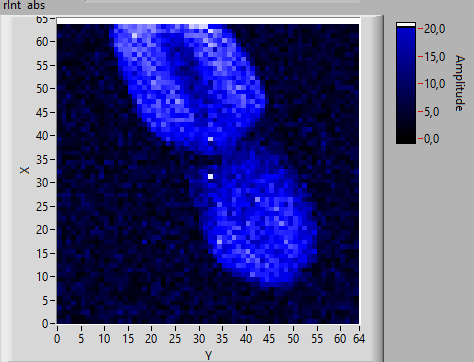
\includegraphics[width=\textwidth]{./Latex images/nut_airgap.png}
        \caption{ vertical scan of peanut}
        \label{fig:nut vertical}
    \end{subfigure}
    \hfill
    \begin{subfigure}[b]{0.45\textwidth}
        \centering
        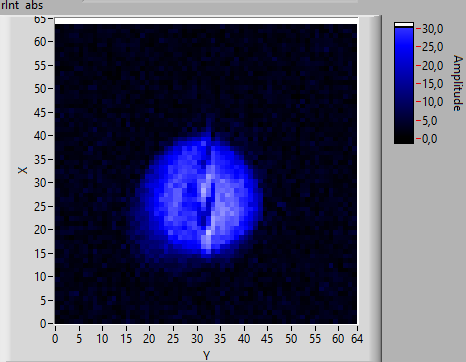
\includegraphics[width=\textwidth]{./Latex images/nut_horizontal.png}
        \caption{horizontal scan of peanut}
        \label{fig:nut horizontal}
    \end{subfigure}
    \vskip\baselineskip
    \begin{subfigure}[b]{0.45\textwidth}
        \centering
        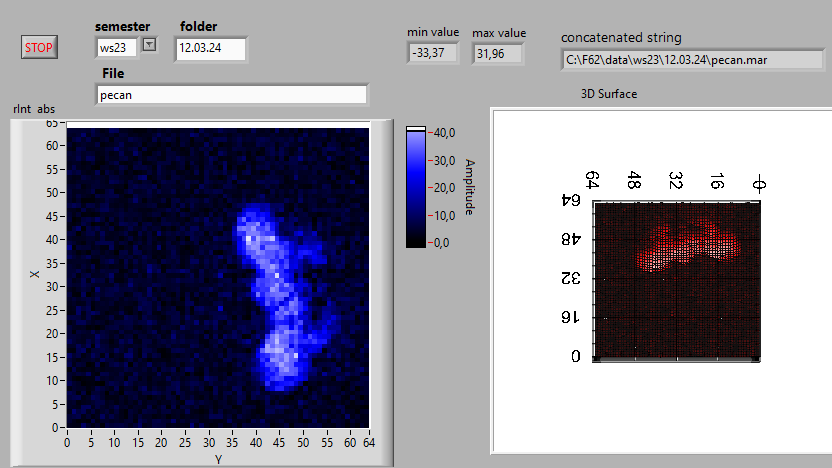
\includegraphics[width=\textwidth]{./Latex images/pecan.png}
        \caption{horizontal scan of pecan}
        \label{fig:pecan}
    \end{subfigure}
    \hfill
    \begin{subfigure}[b]{0.45\textwidth}
        \centering
        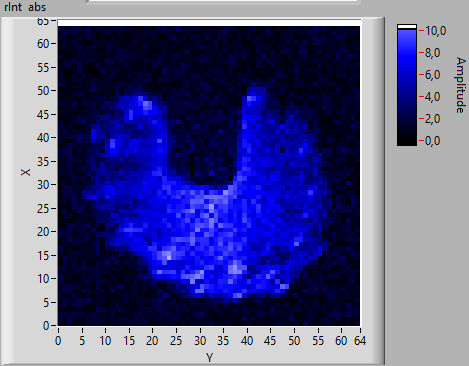
\includegraphics[width=\textwidth]{./Latex images/cellerie.png}
        \caption{horizontal scan of peanut}
        \label{fig:celery}
    \end{subfigure}
    \caption{2D profiles of different objects}
    \label{fig:NMRI}
\end{figure}




